\chapter{Technical Background}
\label{chap:background}

\section{Mathematical Models for the Spread of Infectious Diseases}
\label{sec:sem_background}

Our objective is to estimate the posterior distribution of parameters, $ \btheta $, that govern the dynamics of an outbreak, given the data $ \bY = (\bY_1,\dots,\bY_L) $, which are accrued at a set of discrete observation times, $ \lbrace t_\ell: \ell=1,\dots,L\rbrace $. The data are not independent and typically exhibit complicated temporal (and spatial) dependencies. Therefore, the observed data likelihood in the posterior is not a simple product of independent densities, i.e.,
\begin{align*}
\pi(\btheta|\bY) &\propto\ L(\bY|\btheta)\pi(\btheta) \\
&= \prod_{\ell = 1}^{L} \pi(\bY_\ell|\bY_{1},\dots,\bY_{\ell-1},\btheta)\pi(\btheta) \neq \prod_{\ell = 1}^{L} \pi(\bY_\ell|\btheta)\pi(\btheta).
\end{align*}
Furthermore, the transition density, $ \pi(\bY_{\ell}|\bY_{1},\dots,\bY_{\ell-1}) $, involves a high dimensional integral over an unobserved epidemic process, $ \bX $, 
\begin{equation}
\label{eqn:sem_post}
\pi(\btheta|\bY) \propto \int \prod_{\ell = 1}^{L} \pi(\bY_\ell|\bY_{1},\dots,\bY_{\ell-1},\bX,\btheta)\pi(\bX|\btheta)\pi(\btheta)\rmd\bX.
\end{equation}
This integral is analytically intractable when the state space of $ \bX $ is of even moderate size. Simply put, it is difficult to enumerate how the data could have arisen, given the vastness of possibilities for how an unseen outbreak might have evolved. 

In this dissertation, we will describe the latent epidemic process using continuous--time models that possess the Markov property, meaning that the forward--time evolution of the latent process depends on its history only through its current state. This choice reduces the structure of (\ref{eqn:sem_post}) to that of a hidden Markov model wherein the data are conditionally independent given the latent epidemic process (diagrammed in Figure \ref{fig:semhmm}). The  posterior is 
\begin{align}
\label{eqn:sem_post_hmm}
\pi(\btheta|\bY) &\propto\int \prod_{\ell = 1}^{L} L\left (\bY_\ell|\bX(t_{\ell}),\btheta\right ) \pi\left (\bX(t_\ell)|\bX(t_{\ell-1}),\btheta\right )\pi(\btheta)\rmd\bX.
\end{align}
On its own, this might seem to solve nothing. The integral in (\ref{eqn:sem_post_hmm}) is still analytically intractable, and the state space of $ \bX $ is still too large to easily work with the augmented posterior, 
\begin{equation}
\pi(\btheta,\bX|\bY)\propto L(\bY|\bX,\btheta)\pi(\bX|\btheta)\pi(\btheta).
\end{equation}
However, this choice also creates symmetries in the ways that individuals interact and contribute to the outbreak dynamics. This additional structure is critical in facilitating efficient computation. In the following sections, we present a number of representations for the latent epidemic process, and conclude with a brief overview of computational approaches for inference.  

\begin{figure}[htbp]
	\centering
	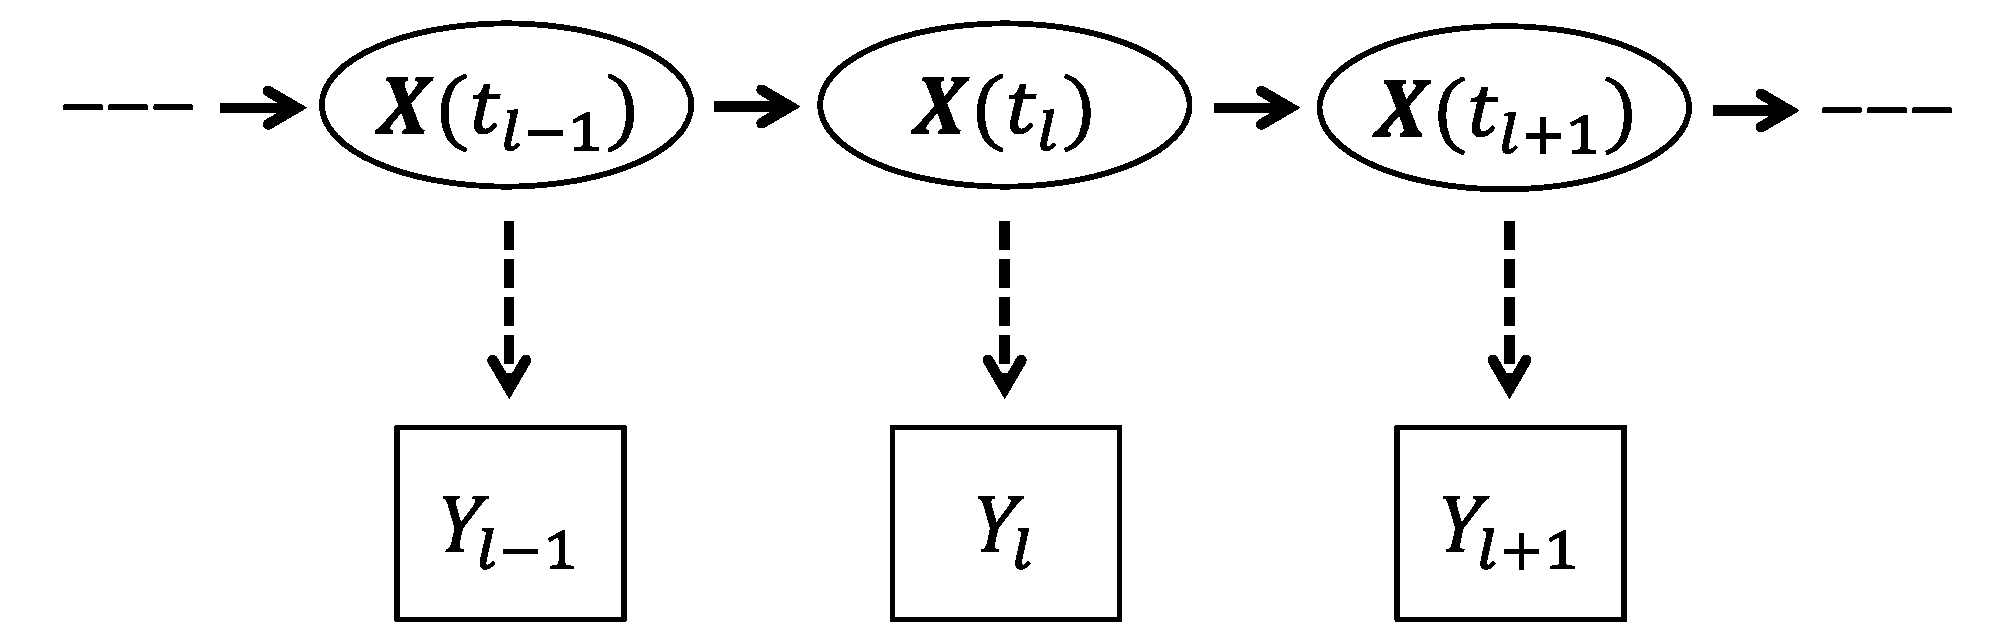
\includegraphics[width=0.5\linewidth]{figures/SEM_HMM}
	\caption[Diagram of a Hidden Markov model.]{Diagram of a Hidden Markov model. The data are conditionally independent given the latent epidemic process.}
	\label{fig:semhmm}
\end{figure}

\subsection{An Agent--Based Susceptible--Infected--Recovered Model}
\label{subsec:sir_individual_mod}
For clarity of exposition, we will present the technical background on epidemic models in terms of the susceptible--infected--recovered (SIR model). Formal treatments that deal with this material in greater generality can be found in \cite{andersson2000stochastic,britton2018,brauer2008compartmental,fuchs2013inference,greenwood2009stochastic,wilkinson2011stochastic}. The SIR model classifies individuals in a population of size $ N $ into one of three infection states: susceptible (S), infected (I), and recovered (R). Individuals are assumed to become infectious immediately upon entering the infected state, and acquire lasting immunity upon recovery. To simplify matters, we will assume the population is closed, meaning that there are no demographic changes or immigration, and that individuals are exchangeable. This latter assumption implies that individuals mix homogeneously and are alike in their infection dynamics. 

The SIR model defines an epidemic process, $ \bX = \lbrace\bX_1,\dots,\bX_N\rbrace $, that collects the subject--level subprocesses, $ \bX_j,\ j=1,\dots,N $, each of which takes values in the state space of disease state labels, $ \mcS_j= \lbrace S,I,R\rbrace $. A realized subject--path is of the form 
\begin{equation}
\bx_j = \left \lbrace\begin{array}{ll}
S,\ & \tau < \tau_I^{(j)},\\
I,\ & \tau_I^{(j)}\leq\tau<\tau_R^{(j)},\\
R,\ & \tau_R^{(j)} \leq \tau,
\end{array}\right .
\end{equation}
where $ \tau_I^{(j)} $ and $ \tau_{R}^{(j)} $ are the infection and recovery times for subject $ j $, and are possibly infinite (Figure \ref{fig:subjectsamplepaths}). The state space of $ \bX $ is  $ \mcS = \lbrace S,I,R\rbrace^N $, the Cartesian product of subject--level state labels. We denote by $ \bX(\tau) = \left (\bX_1(\tau),\dots,\bX_N(\tau)\right ) $ the state of $ \bX $ at time $ \tau $, and by $ \bX(\tau^+) $ the state just after time $ \tau $. 

\begin{figure}[htbp]
	\centering
	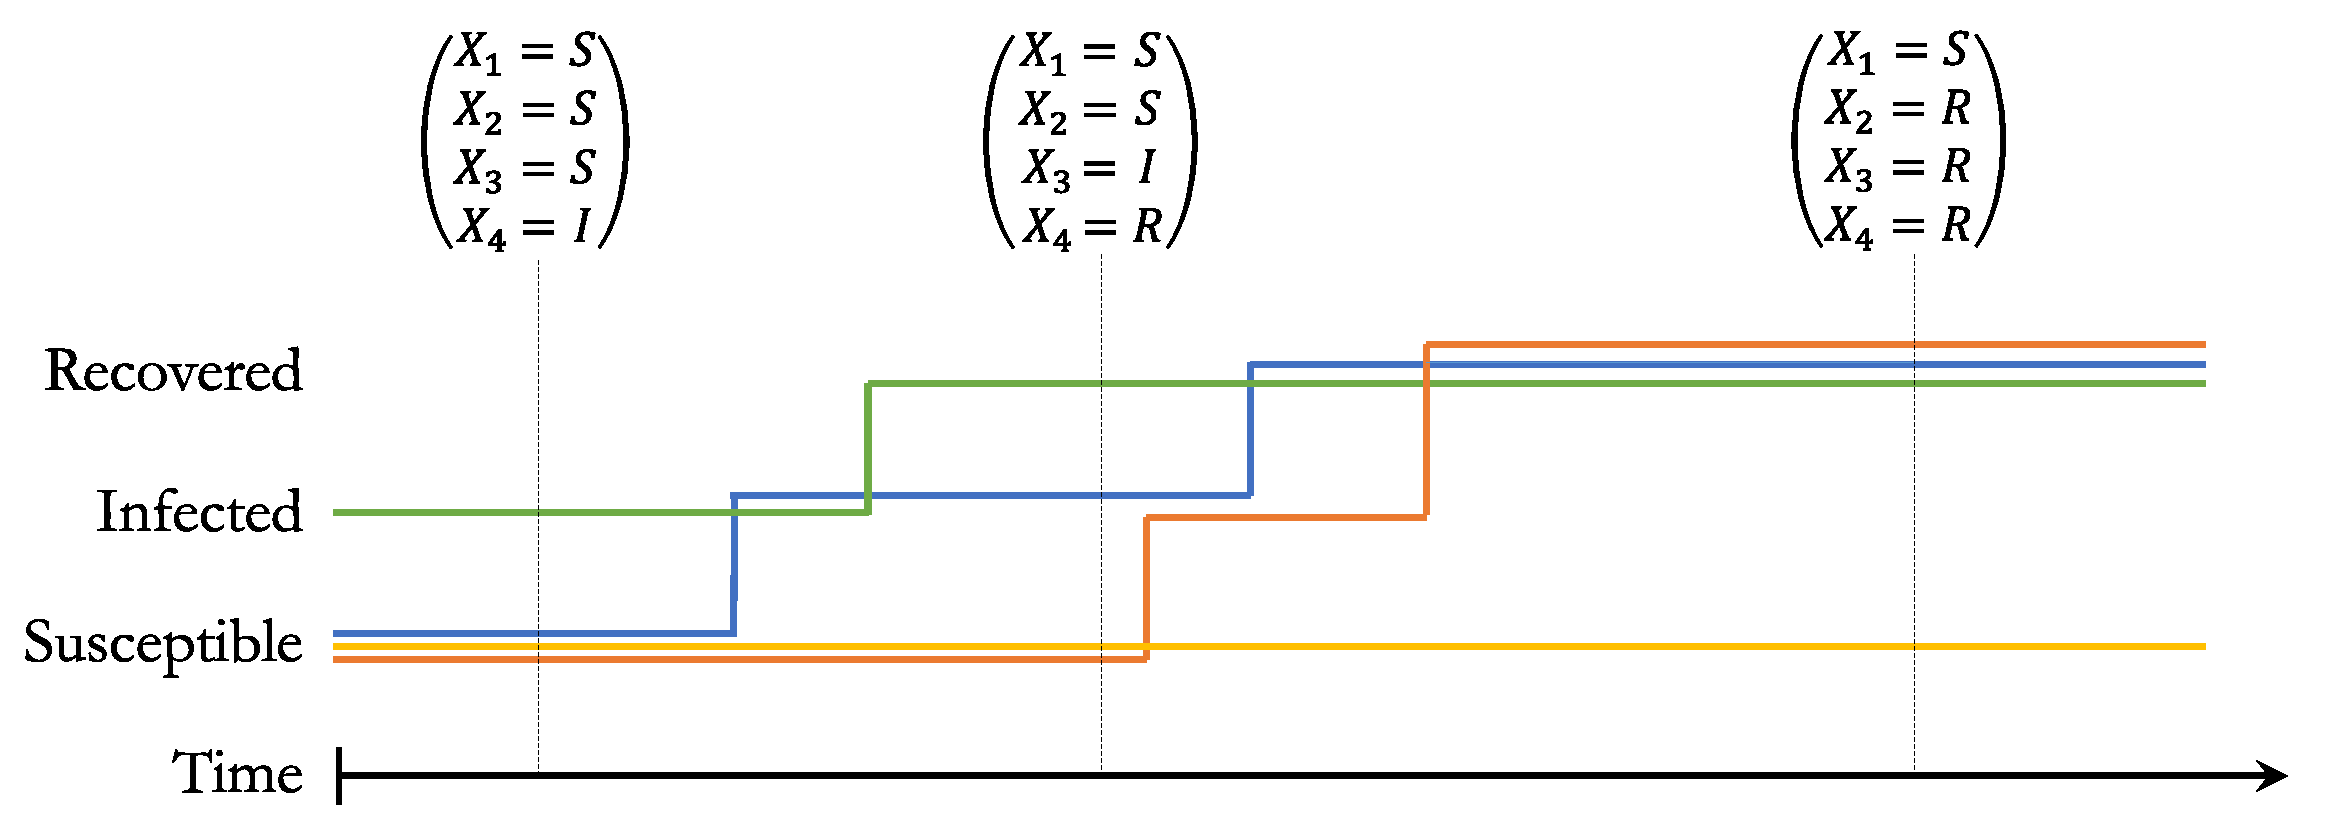
\includegraphics[width=0.8\linewidth]{figures/subject_sample_paths}
	\caption[Diagram of subject--level SIR paths.]{Diagram of subject--level paths (colored lines) for an SIR model in a population of size $ N=4 $. Individuals transition through infection states continuously in time. The epidemic process is defined in terms of the infection states of individuals in the population.}
	\label{fig:subjectsamplepaths}
\end{figure}

The waiting times between subject--level transition events are typically taken to be exponentially distributed. This will allow us to take advantage of several useful properties of exponential random variables (List \ref{list:exp_props}, see \cite{wilkinson2011stochastic} for proofs). Critically, this choice also implies that $ \bX $ evolves as a continuous--time Markov chain (CTMC) with transition rate from configuration $ \bX $ to $ \bX^\prime $, differing only in the state of a single subject, given by
\begin{equation}
\lambda_{\bX,\bX^\prime} = \left \lbrace \begin{array}{rl}
\beta I,\ &\text{if } \bX\ \text{and } \bX^\prime\ \text{differ only in subject }j \text{, with }\bX_j=S\text{, and }\bX_j^\prime=I,\\
\mu,\ &\text{if } \bX\ \text{and } \bX^\prime\ \text{differ only in subject }j \text{, with }\bX_j=I\text{, and }\bX_j^\prime=R,\\
0,\ & \text{for all other configurations }\bX\ \text{and }\bX^\prime.
\end{array}\right.
\end{equation}
with per--contact infection rate,  $ \beta $, and recovery rate, $ \mu $. The quantity, $ 1/\mu $, is interpreted as the mean infectious period duration. That $ \bX $ is a \textit{Markov} process means that its forward--time evolution depends on its history only through its current state, i.e.,
\begin{equation}
\label{eqn:sir_markov}
\Pr\left (\bX(\tau + \dtau) = \bx^\prime | \lbrace\bX(\tau) = \bx,\ \tau\in[0,\tau]\rbrace, \btheta\right ) = \Pr\left (\bX(\tau + \dtau) = \bx^\prime | \bX(\tau) = \bx,\btheta\right ),
\end{equation}
where $ \bx^\prime,\bx \in \mcS$. $ \bX $ is \textit{time--homogeneous} since the rates of transition between configurations in the state space of $ \bX $ are constant over time. 

Let $ \btau = \lbrace\tau_0,\dots,\tau_{K+1}\rbrace $, be the (ordered) set of $ K $ infection and recovery times of all individuals along with the endpoints of the time period $ [\tau_0,\ \tau_{K+1}] $. Let $ \ind{\tau_k \corresponds I} $ and $ \ind{\tau_k \corresponds R} $ indicate whether $ \tau_k $ is an infection or recovery time, and let $ \btheta = (\beta, \mu, \bX_0) $ denote the vector of parameters, including the initial state of $ \bX $ at time $ \tau_0 $. The CTMC likelihood of $ \bX $ over $ [\tau_0,\ \tau_{K+1}] $ is a product of exponential waiting time densities,
\begin{align} 
\label{eqn:sir_subj_likelihood}
L(\bX| \btheta) &= \prod_{k = 1}^{K}\left \lbrace \left [\beta I_{\tau_k}\times\ind{\tau_k \corresponds I} + \mu\times\ind{\tau_k \corresponds R}\right ] \exp{\left [-\left (\tau_k - \tau_{k-1}\right )\left (\beta I_{\tau_k} S_{\tau_k} + \mu I_{\tau_k}\right )\right ]}\right \rbrace \nonumber \\
& \hspace{0.2in} \times \exp \left [-\left (t_L - \tau_K\right )\left (\beta I_{\tau_K^+}S_{\tau_K^+} + \mu I_{\tau_K^+}\right )\right ]. 
\end{align}

\begin{framed}
	\begin{itemize}
		\begin{lstlisting}[caption={Useful properties of exponential random variables.},label={list:exp_props}]
		\end{lstlisting}
		\item (Memoryless property) If $ Z\sim\mr{Exp}(\lambda)$, then $ \forall t,\dt\geq0 $  we have \begin{equation}\label{eqn:memoryless_prop}
		\Pr(Z > t+\dt | Z>t) = \Pr(Z>\dt).
		\end{equation}
		\item (Racing exponentials) If $ Z_i\sim\mr{Exp}(\lambda_i),\ i=1,\dots,n $, are independent, then \begin{equation}\label{eqn:racing_exponentials}
		\underset{i}{\mr{min}}(Z_i) \sim \mr{Exp}\left (\lambda = \sum_i\lambda_i\right ).
		\end{equation}
		\item (Index of minimum) If $ Z_i\sim\mr{Exp}(\lambda_i),\ i=1,\dots,n $, are independent, then the index $ k $ of the minimum of $ Z_i $ is a random variable with probability mass function \begin{equation}\label{eqn:ind_of_min}
		\Pr(k|Z_k = \min(Z_1,\dots,Z_n)) = \frac{\lambda_k}{\sum_j\lambda_j}.
		\end{equation} 
		\item (Minimum is independent of its index) If $ Z_i\sim \mr{Exp}(\lambda_i)$ are independent, then $ M = \underset{i}{\mr{min}}(Z_i) $, which is the minimum of $ Z_i $, and $ I $, the index of the minimum taking value $ I=k $ if $ Z_k=M$, are independent.
	\end{itemize}
\end{framed}

\subsection{A Population--Level Susceptible--Infected--Recovered Model}
\label{subsec:sir_population_mod}
The subject--level SIR model is equivalent to an aggregated SIR model, expressed in terms of compartment counts \cite{allen2008introduction, andersson2000stochastic}. This equivalence derives from two properties of Markov processes, \textit{lumpability} and \textit{commutativity}. The population--level SIR model is usually presented for computational reasons since discarding the subject labels associated with infections and recoveries substantially reduces the computational burden of caching subject--level paths. We refer to \cite{tian2006lumpability} for a more formal presentation of the following discussion. 

Given a Markov process, $ \bX $ with state space $ \mcS = \lbrace s_1,\dots,s_P\rbrace $ and initial probability vector $ \pi $, we define another process, $ \overline{\bX} $ on the state space $ \overline{\mcS} = \lbrace S_1,\dots,S_\mathcal{L}\rbrace $, which is a \textit{partition} of $ \mcS $. In our setting, the partitioning will map a configuration in $ \mcS $ to a set in $ \overline{\mcS} $ by counting the number of people in each model compartment. The jump chain of the new process is obtained by partitioning the jump chain of the complete process. We want to establish conditions under which $ \overline{\bX} $ is stochastically coupled to $ \bX $. 

Suppose the initial distribution of $ \overline{\bX}(t_0) $, induced by the distribution of $ \bX(t_0) $, is \begin{equation*}
\Pr(\overline{\bX}(t_0) = S_i) = \mathrm{Pr}_\pi(\bX(t_0) \in S_i)
\end{equation*}
and that its transition probabilities are
\begin{equation*}
\Pr(\overline{\bX}(t+\Delta t) = S_j | \overline{\bX}(t)=\overline{\bx}(t^\prime), t^\prime \leq t) = \Pr(\overline{\bX}(t+\Delta t) \in S_j | \bX(t)=\bx(t^\prime), t^\prime \leq t),
\end{equation*}
where $ \overline{\bx}(t^\prime) $  and $ \bx(t^\prime) $ denote the paths of the complete Markov process and the new process. We say that the complete Markov process is \textit{lumpable} with respect to a partition, $ \overline{\mcS} $, of its state space if lumping the complete process results in a Markov process with respect to the lumped state space for every choice of $ \pi $ whose transition probabilities do not depend on $ \pi $. We refer to the process obtained by lumping as the \textit{lumped} Markov jump process (MJP). We say that the complete process is \textit{commutative} with respect to lumping if the set of jump chains obtained by applying the lumping to jump chains of the complete MJP are equal in distribution to jump chains of the lumped MJP.

Let $ S_A $ and $ S_B $ be elements of $ \overline{\mcS} $, i.e., sets of states $ s_j \in \mcS $. The rate matrix of a CTMC is lumpable if
\begin{equation*}
\sum_{s_b \in S_B}\lambda_{s_a,s_b} = \sum_{s_b \in S_B}\lambda_{s_c,s_b}
\end{equation*}
for any pair of sets $S_A,S_B \in \overline{\mcS} $ and any pair of states  $(s_a, s_c) \in S_A$. A Markov process $ \bX $ is lumpable with respect to a partition of its state space if and only if its rate matrix is lumpable. Lumpability implies that transition probabilities for the lumped chain can be computed based on the lumped rate matrix  \cite{tian2006lumpability}.

Suppose $ \bX $ is lumpable with respect to the partition $ \overline{\mcS} $ of $ \mcS $. Then $ \bX $ is commutative with respect to the partition if and only if the rate matrix of $ \bX $ satisfies
$$\lambda_{s_a,s_b} = 0,\ \text{if}\ s_a,s_b\in S_A,\ \text{and}\ s_a\neq s_b. $$ In our context, commutativity means that the transition rate is zero between different configurations $ \bx_a $ and $ \bx_b $ with equal compartment counts. Commutativity implies that lumped quantities of interest for $ \bX $, such as transition rates or transition probabilities, can be equivalently computed based on $ \bX $, or based on the lumped process, $ \overline{\bX} $ \cite{tian2006lumpability}. 

\begin{figure}
	\centering
	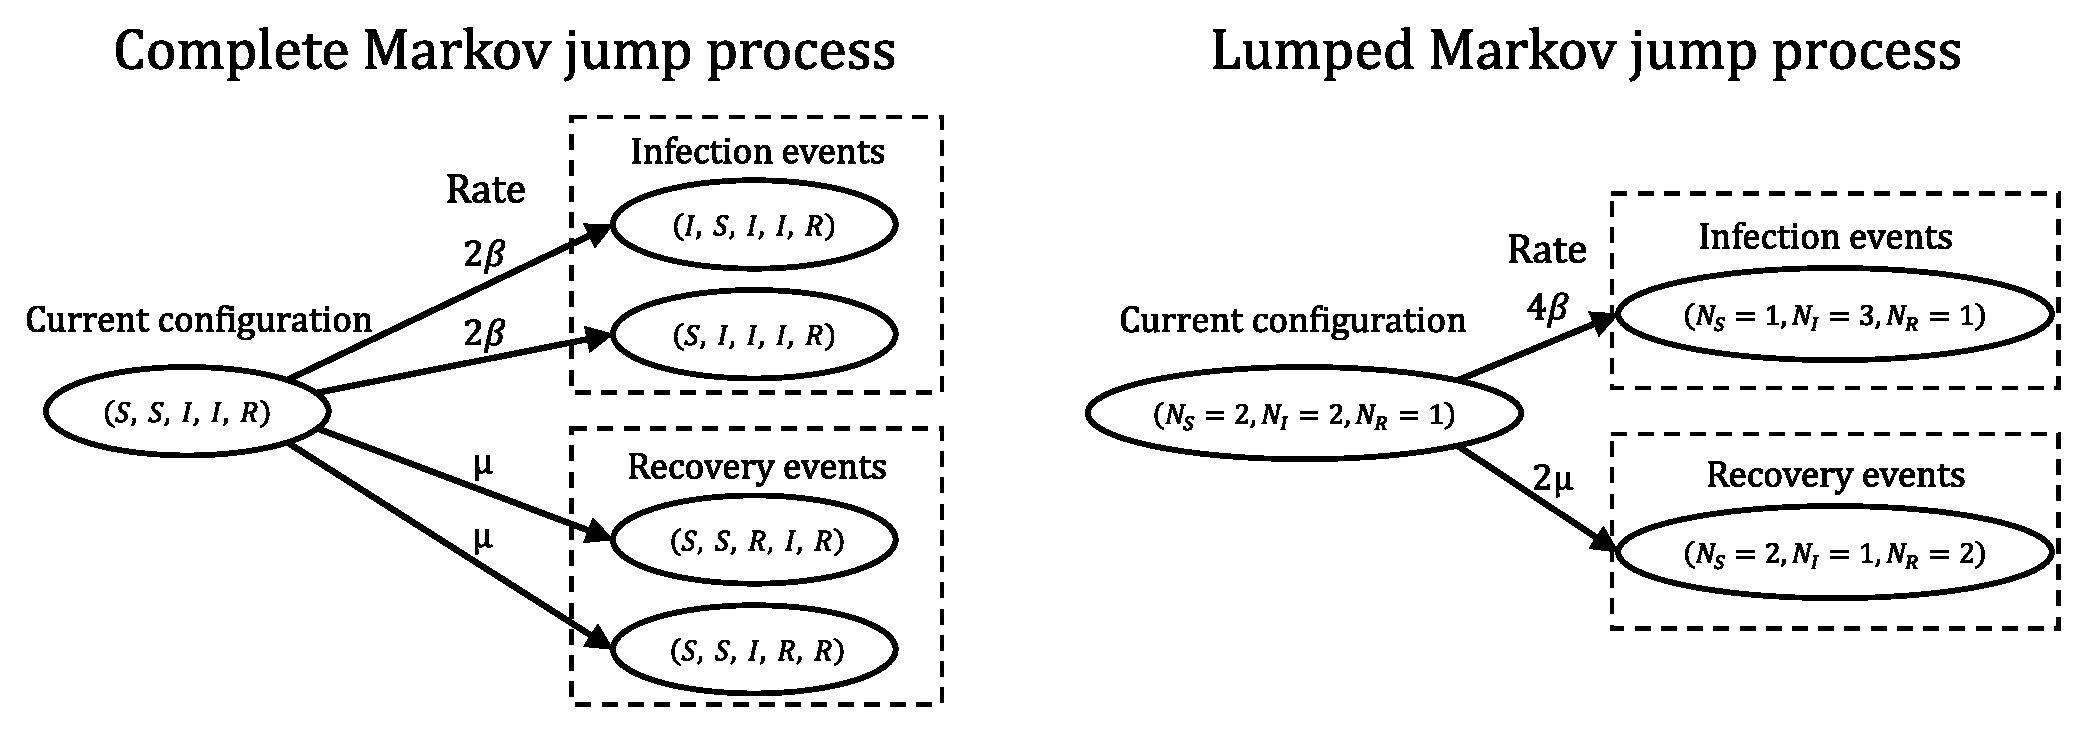
\includegraphics[width=\linewidth]{figures/SIR_representations}
	\caption[Individual and lumped representations of SIR dynamics.]{Complete and lumped representations of SIR dynamics in a population of five individuals. The per--contact infectivity rate, $ \beta $, and the recovery rate, $ \mu $, parameterize exponential waiting time distributions between transition events. The complete Markov jump process evolves on the state space of subject state labels, $ \mcS = \lbrace S,I,R\rbrace^N $, with dynamics determined by the subject--level transition rates. Each susceptible may contact two infected individuals, while each infected individual recovers independently. The lumped process evolves on the state space of compartment counts, $ \widebar{\mcS} = \lbrace N_S,N_I,N_R:\ N_S + N_I+N_R=N\rbrace $, with dynamics determined by lumped transition rates. The waiting time distributions between transitions are derived by noting that if $ \tau_1\sim \exp(\lambda_1) $ and $ \tau_2\sim\exp(\lambda_2) $, then $ \tau_{\min} = \min(\tau_1,\tau_2)\sim\exp(\lambda_1+\lambda_2) $.}
	\label{fig:sirrepresentations}
\end{figure}

Turning back to the SIR model, we defined the epidemic process, $ \bX(\tau) = (\bX_1,\dots,\bX_N)$, with state space $ \mcS = \lbrace S, I, R\rbrace^N $. Let $ \bx = (x_1,\dots,x_N) $ denote a configuration of the state labels (e.g. $ \bx = (S, I, S, R, I) $), and let $$ \overline{\bx} = h(\bx) = \left (l=\sum_{i=1}^N\ind{x_i = S},m=\sum_{i=1}^N\ind{x_i=I},n = \sum_{i=1}^N\ind{x_i=R}\right ) $$ be the corresponding vector of compartment counts. The lumped state space is 
$$ \overline{\mcS} = \left \lbrace \overline{\bx} = (l,m,n): l,m,n \in \lbrace0,\dots,N\rbrace,\  l+m+n = N \right \rbrace, $$ 
which partitions $ \mcS $ by summing the number of individuals in each disease state. 

The population--level SIR model expressed in terms of compartment counts, $ \overline{\bX} = (S, I, R) \in \overline{\mcS} $ (depicted in Figure \ref{fig:sirrepresentations}), evolves as a CTMC on the lumped state space $ \overline{\mcS} $ with transition rates
\begin{equation*}
\begin{array}{cc}
\underline{\text{Transition}} & \underline{\text{Lumped Rate}} \\
(S,I,R) \longrightarrow (S-1,I+1,R) & \beta S I ,\\
(S,I,R) \longrightarrow (S,I-1,R+1) & \mu I .
\end{array}
\end{equation*}
To see how we arrive at these rates, note that in a population with $ S $ susceptibles, each of whom is independently infected at rate $ \beta I $, the time until the first infection is exponentially distributed with rate $ \lambda_{SI} = \beta SI $ by the racing exponentials property (\ref{eqn:racing_exponentials}). Similarly, the time to the first recovery in a population with $ I $ infected individuals is exponentially distributed with rate $\lambda_{IR} = \mu I $. Note that the mean infectious period duration is still $ 1/\mu $, as it was in the case of the subject--level SIR model.

Again, let $ \btau = \lbrace\tau_0,\dots,\tau_{K+1}\rbrace $, be the (ordered) set of $ K $ infection and recovery times, along with the endpoints of the time period $ [\tau_0,\ \tau_{K+1}] $ over which the outbreak is modeled. We indicate by $ \ind{\tau_k \corresponds I} $ and $ \ind{\tau_k \corresponds R} $ whether $ \tau_k $ is an infection or recovery time, and let $ \btheta = (\beta, \mu, \overline{\bX}_0) $ denote the vector of parameters, including the initial state of $ \overline{\bX} $ at time $ \tau_0 $. The CTMC likelihood of $ \overline{\bX} $ over $ [\tau_0,\ \tau_{K+1}] $ is a product of exponential waiting time densities,
\begin{align} 
\label{eqn:sir_pop_likelihood}
L(\overline{\bX}| \btheta) &= \prod_{k = 1}^{K}\left \lbrace \left [\beta S_{\tau_k} I_{\tau_k}\times\ind{\tau_k \corresponds I} + \mu I_{\tau_k}\times\ind{\tau_k \corresponds R}\right ] \exp{\left [-\left (\tau_k - \tau_{k-1}\right )\left (\beta I_{\tau_k} S_{\tau_k} + \mu I_{\tau_k}\right )\right ]}\right \rbrace \nonumber \\
& \hspace{0.2in} \times \exp \left [-\left (t_L - \tau_K\right )\left (\beta I_{\tau_K^+}S_{\tau_K^+} + \mu I_{\tau_K^+}\right )\right ]. 
\end{align} 

\subsection{A Brief Review of CTMCs}
\label{subsec:ctmc_overview}

We briefly digress from our discussion of epidemic models to review some basic properties of CTMCs in a bit more generality. The following discussion is not intended to be comprehensive, but rather to provide an overview of some results that will be useful in this dissertation. We refer to \cite{bremaud1999markov,fuchs2013inference,guttorp1995stochastic,wilkinson2011stochastic} for more complete and rigorous discussions of the following material. For simplicity, we will focus on CTMCs with finite state spaces. 

The forward--time evolution of a CTMC is described by its transition kernel $$\Pr(\bX(\tau^\prime) = \bx^\prime | \bX(\tau) = \bx) = \bP_{\bx,\bx^\prime}(\tau,\tau^\prime),$$
where $ \bx,\bx^\prime\in\mcS $ and $ 0\leq\tau\leq\tau^\prime $. The transition kernel only depends on the time--elapsed when the process is time--homogeneous $ \bP_{\bx,\bx^\prime}(\tau,\tau^\prime) = \bP_{\bx,\bx^\prime}(|\tau^\prime - \tau|)$. We will use the shorthand notation $ \bP(\tau) $ to simply denote the transition kernel for a time--homogeneous CTMC over a time interval of length $ \tau $, and $ P_{ij}(\tau) $ to denote its $ i,j $ element. 
In matrix form, the transition kernel, $ \bP(\tau) $, is an $ r\times r $ stochastic matrix, where $ r = |\mcS| $, the rows of $ \bP(\tau) $ sum to one, and $ P_{ii}(\tau) = -\sum_{j\neq i}P_{ij}(\tau)$. 
Trivially, $ \bP(0) = \bI $, i.e., there are no state changes in a time interval of zero length, almost surely. By the Markov property, the probability of transitioning from state $ i $ to state $ k $ in time $ s+t $ is 
\begin{equation}
\label{eqn:chapman_kolmogorov}
P_{ik}(s+t) = \sum_{j\in\mcS}P_{ij}(s)P_{jk}(t),
\end{equation}
or in matrix form, $$\bP(s+t) = \bP(s)\bP(t).$$
Equation (\ref{eqn:chapman_kolmogorov}) is known as the \textit{Chapman--Kolmogorov} master equation. 

The transition rate matrix (or \textit{infinitesimal generator}) of $ \bX $ is defined as the derivative of $ \bP(\tau) $ at $ \tau = 0 $, i.e.,
\begin{align*}
\label{eqn:ctmc_generator}
\bLambda &= \underset{\dtau \rightarrow 0}{\lim}\frac{\bP(\dtau) - \bP(0)}{\dtau} \\
&= \underset{\dtau \rightarrow 0}{\lim}\frac{\bP(\dtau) - \bI}{\dtau}, \\
\shortintertext{which implies that the infinitesimal transition matrix is} \bP(\dtau) &= \bI + \bLambda\dtau.
\end{align*}
Thus, for example, the infinitesimal transition probabilities for the population--level SIR model are
\begin{align*}
\Pr\left (\bX(\tau+\dtau) = (S-1, I+1, R) | \bX(\tau) = (S,I,R)\right ) &= \beta SI\dtau + o(\dtau), \\
\Pr\left (\bX(\tau+\dtau) = (S, I-1, R+1) | \bX(\tau) = (S,I,R)\right ) &= \mu I\dtau + o(\dtau).
\end{align*}
The transition probability matrix over an interval of arbitrary length, $ \tau $, solves the matrix differential equation,  \begin{equation}\label{eqn:kolmogorov_forward}
\deriv{}{\tau}\bP(\tau) = \bLambda P(\tau),\hspace{0.2in} s.t.\  \bP(0) = \bI.
\end{equation} 
Thus, $ \bP(\tau) = \exp(\bLambda\tau) $, can be computed using the matrix exponential. There are many ways to compute the matrix exponential \cite{moler2003nineteen}. We will typically do so by diagonalizing $ \bLambda $ and exponentiating the eigenvalues. Section \ref{sec:mtx_exp} outlines this procedure in two separate cases: when $ \bLambda$ has real--valued eigenvalues, and also when the eigenvalues are complex. Equation (\ref{eqn:kolmogorov_forward}) is known as the \textit{forward} Kolmogorov equation, and is obtained by computing the derivative
\begin{align*}
\deriv{}{\tau}\bP(\tau) &= \frac{\bP(\tau + \dtau) - \bP(\tau)}{\dtau} \\
&= \frac{\bP(\dtau)\bP(\tau) - \bP(\tau)}{\dtau} \\
&= \frac{\bP(\dtau) - \bI}{\dtau}\bP(\tau)\\
&= \bLambda \bP(\tau).
\end{align*}
The \textit{backward} Kolmogorov equation is similarly obtained by
\begin{align}
\deriv{}{\tau}\bP(\tau) &= \frac{\bP(\tau + \dtau) - \bP(\tau)}{\dtau} \nonumber \\
&= \frac{\bP(\tau)\bP(\dtau) - \bP(\tau)}{\dtau} \nonumber \\
&= \bP(\tau)\frac{\bP(\dtau) - \bI}{\dtau}\nonumber\\
&= \bP(\tau)\bLambda .
\end{align}

\subsection{Large Population Approximations}
\label{subsec:sem_approximations}

It is often infeasible to work with the CTMC formulation of a SEM when modeling an outbreak in a large population, particularly when working within a Bayesian MCMC framework. The cardinality of model's state space grows polynomially in the population size. This makes it difficult to efficiently sample from the posterior or to explore the likelihood surface, even when fitting SEMs with relatively simple dynamics. A second challenge is that as the population size grows, so too do the numbers of transition events. Hence, repeatedly evaluating the likelihoods (\ref{eqn:sir_subj_likelihood}) and (\ref{eqn:sir_pop_likelihood}) is prohibitively expensive. 

Two commonly used approximations of the MJP representation of a SEM are through a system of ordinary differential equations (ODEs) and through a system of stochastic differential equations (SDEs). We will not go into detail on the derivations of these representations, except to give some intuition about the conditions under which they are appropriate, and refer to \cite{allen2017primer,greenwood2009stochastic} for more detailed overviews. 

We presented the MJP representation of the SIR model as an \textit{extensive}, $ \bX $, where transition events led to jumps of size one in the compartment counts. We could have equivalently defined the model in terms of an \textit{intensive} process, $ \bXtil = \bX / N = (S/N,I/N,R/N) $, where transition events led to jumps of size $ 1/N $. As $ N\longrightarrow \infty$ , it becomes reasonable to consider approximating $ \bXtil $ by a process with continuous sample paths. The large population stochastic \textit{approximation} is the solution to an It\^{o} diffusion whose sample paths are continuous but nowhere differentiable. The infinite population deterministic functional \textit{limit} solves a system of ODEs and has smooth sample paths. We will present extensive forms of the SDE and ODE models, which are obtained by simply rescaling the intensive processes from which the approximations derive. 

\subsubsection{Deterministic representation as a system of ODEs}
\label{subsec:deterministic_models}

In the infinite population limit, sample paths of the MJP converge pointwise to their deterministic functional limit, which is given by the solution to a system of ordinary differential equations \cite{greenwood2009stochastic,kurtz1981approximation}. For the SIR model, $ \bX(t)  = \lim_{N \rightarrow \infty} \E(N\bXtil(t))$ is the solution to the following system of ODEs, subject to the initial constraint that $ \bX(\tau_0) = \bx_0 $:
\begin{align*}
\deriv{S}{t} = -\beta S I,\hspace{0.25in} 
\deriv{I}{t} = \beta S I - \mu I,\hspace{0.25in} 
\deriv{R}{t} = \mu I.
\end{align*}
The state space of the ODE representation of the SIR model is $$ \mcS^R =  \lbrace(j,k,l):\ j,k,l\in[0,N],\  j+k+l = N\rbrace. $$ Note that the ODE model implies that if $ I(\tau) > 0 $ at any time $ \tau $, then $ I(\tau) > 0\ \forall\ \tau\in[0,\infty)$. Therefore, the ODE model is not appropriate if we are interested in answering questions about the stochastic emergence or extinction of an outbreak.

ODE formulations of SEMs are particularly useful, in part, because they more easily lend themselves mathematical analysis. One important quantity that is straightforwardly derived for ODE models is the basic reproduction number, $ R_0 $, which is interpreted as the expected number of secondary infections attributable to a single index case in an otherwise susceptible population (of infinite size). The basic reproduction number can be related to both the final size distribution and to the probability of a major outbreak \cite{allen2017primer,greenwood2009stochastic,miller2012note}. The formulation of $ R_0 $ is more complicated for stochastic models, though it can be derived from a branching process approximation for the early behavior of an outbreak \cite{allen2008introduction}. In the case of deterministic models, $ R_0 $ is calculated as the spectral radius of the next generation matrix (NGM) for the linearized system of ODEs at the disease free equilibrium (DFE) \cite{diekmann2009construction,van2017reproduction}. Other methods exist, e.g., by analyzing the survival function or by fitting phenomenological models when the growth rate of the outbreak is observed to be subexponential \cite{van2017reproduction}.

As an example, we will demonstrate the NGM method for calculating $ R_0 $ for an outbreak with SIR dynamics where a fraction of the population, $ p_v $, is vaccinated and vaccine efficacy (VE)  modifies the per--contact rate of infection (VE for susceptibility: $ \nu_s $), the infectiousness of carriers (VE for infectiousness: $ \nu_i $), and the rate of recovery (VE for recovery: $ \nu_r $). We will write $ N^{u} = (1-p_v)N $ and $ N^{v} = p_vN $. The DFE is \begin{small}
	$$ \bX_{DFE} =  \left (S^{(u)}_{DFE} = (1 - p_v)N,\ I^{(u)}_{DFE} = 0,\  R^{(u)}_{DFE} = 0,\ S^{(v)}_{DFE} = p_vN,\ I^{(v)}_{DFE} = 0,\ R^{(v)}_{DFE} = 0\right ). $$
\end{small} 
The linearized system of ODEs at the DFE is 
\begin{align*}
\deriv{I^{(u)}}{t} &= \beta \left (I^{(u)} + \nu_iI^{(v)}\right )N^{(u)} - \mu I^{(u)},\hspace{0.2in} 
\deriv{I^{(v)}}{t} = \beta \nu_s\left (I^{(u)} + \nu_iI^{(v)}\right )N^{(v)} - \mu\nu_r I^{(v)}.
\end{align*}	
The NGM is constructed as $\bK=-\bT\bSigma^{-1}$, where $bT$ gives the rates of infectious contact between states at infection, $ I^{(u)} $ and $ I^{(v)} $, and $\bSigma$ contains the recovery rates out of states at infection. Here,
\begin{align*}
\bT &= \kbordermatrix{ & I^{(u)} & I^{(v)} \\
	I^{(u)} & \beta N^{u} & \nu_i\beta N^u\\
	I^{(v)} & \nu_s \beta N^{v} & \nu_s\nu_i\beta N^v}, & &\hspace{-2in}
\bSigma = \kbordermatrix{ & I^{(u)} & I^{(v)} \\
	I^{(u)}&-\mu & 0 \\
	I^{(v)}& 0 & -\mu\nu_r},\\
&\hspace{1.25in} \bK =\kbordermatrix{ & I^{(u)} & I^{(v)} \\
	I^{(u)} & \frac{\beta N^{u}}{\mu} & \frac{\nu_i\beta N^u}{\nu_r\mu}\\
	I^{(v)} & \frac{\nu_s \beta N^{v}}{\mu} & \frac{\nu_s\nu_i\beta N^v}{\nu_r\mu}}.
\end{align*}
Thus, $$ R_0 = \sigma(K) = \frac{1}{2}\left (Tr(K) + \sqrt{Tr(K)^2 - 4\det(K)}\right )  = \frac{\beta N^{u}}{\mu} + \frac{\nu_s\nu_i\beta N^v}{\nu_r\mu}.$$

\subsubsection{Diffusion approximations of Markov Jump Processes}
\label{subsubsec:diff_approx}

We will give the diffusion approximation for the SIR model after a, somewhat colloquial, review of diffusions based on material in \cite{fuchs2013inference,oksendal2003stochastic,schnoerr2017approximation,wilkinson2011stochastic}. We begin with the SDE \begin{equation}
\deriv{\bX_t}{t} = \bmu(\bX_t,t) + \bSigma(\bX_t,t)\bZ_t,\hspace{0.1in} t\geq s;\hspace{0.1in} \bX_x = \bx,\end{equation}
with \textit{drift vector} $ \bmu:\mathbb{R}^d\rightarrow\mathbb{R}^d $ and  \textit{diffusion matrix} $ \bSigma:\mathbb{R}^d\rightarrow \mathbb{R}^d\times\mathbb{R}^d $, which are interpretable as the infinitesimal first and second moments of the process innovations. $ \bZ_t $ is $ d $--dimensional Gaussian white noise. We denote by $ \rmd\bW_t = \bZ_t\dt$ standard $ d $--dimensional Brownian motion (see \cite{oksendal2003stochastic} for a formal definition). An \textit{It\^{o} diffusion} is a stochastic process, $ (\bX_t)_{t\geq0} $, that satisfies the It\^{o} stochastic integral equation
\begin{equation}
\bX_t = \bX_0 + \int_0^t\bmu(\bX_t,t)\dt + \int_0^t\bSigma(\bX_t,t)\rmd\bW_t,\end{equation}
which we can express equivalently in differential form,
\begin{equation}
\label{eqn:general_sde}
\rmd\bX_t = \bmu(\bX_t,t)\dt + \bSigma(\bX_t,t)\rmd\bW_t.
\end{equation}
The SDE (\ref{eqn:general_sde}) can be interpreted as the limit of a difference equation, $ \Delta\bX_t = \bmu(\bX_t,t)\Delta t + \bSigma(\bX_t,t)\Delta\bW_t $, with infinitely small time steps, $ \Delta t \rightarrow 0$. Hence, we can simulate approximate sample paths using an \textit{Euler--Maruyama} scheme by taking $ \Delta t = \epsilon>0 $ and sampling the innovations, $ \Delta\bX_t$, according to
$$\Delta\bX_t\sim MVN\left (\bmu(\bX_t,t)\Delta t,\ \bSigma(\bX_t,t)\bSigma(\bX_t,t)^T\Delta t\right ).$$

Given a $ d $--dimensional It\^{o} process of the form (\ref{eqn:general_sde}), \textit{It\^{o}'s lemma} gives a formula for the SDE satisfied by a transformed process \cite{oksendal2003stochastic}. Let $ g(\bx, t) = \left (g_1(\bx,t),\dots,g_p(\bx,t)\right ) $ be a twice continuously differentiable map from $ \mathbb{R}^d\times[0,\infty)\rightarrow\mathbb{R}^p $. Then the transformed process, $ \bY(\bW,t) = g(\bX_t, t)$, is also an It\^{o} process with component $ Y_k,\ k=1,\dots,p $, given by
$$\rmd Y_k, = \pdiv{g_k}{t}(\bX, t) + \sum_i\pdiv{g_k(\bX,t)}{x_i}\rmd X_i + \frac{1}{2}\sum_i\sum_j\pdiv{^2g_k(\bX,t)}{x_i\partial x_j}\rmd X_i\rmd X_j,$$
where $ \rmd W_i\rmd W_j = \dt\rmd W_i = \rmd W_i\dt = 0 $ and $ \rmd W_i\rmd W_i = \dt. $

The SDE approximation of a density dependent MJP can be rigorously derived in a number of ways. These include proving the convergence of the MJP Kolmogorov master equation to its SDE counterpart, convergence of the infinitesimal generator, and through a number of different system size expansions applied to the master equation \cite{fuchs2013inference}. An intuitive approach yielding an equivalent result, referred to as the \textit{Langevin approach}, postulates that the SDE approximation is obtained by matching the infinitesimal moments of the diffusion to those of the MJP \cite{fuchs2013inference,gillespie2000chemical,wallace2012linear}. 

We proceed by approximating the numbers of infections and recoveries in a small time interval, $ (t, t+\dt] $. Suppose that we can choose $ \dt $ so that the following \textit{leap} conditions hold:
\begin{enumerate}
	\item $ \dt $ is sufficiently \textit{small} that the $ \bX^c $ is essentially unchanged over $ (t,t+\dt] $, so that the rates of infections and recoveries, $ \blambda\left (\bX^c(t)) = (\beta S(t)I(t),\ \mu I(t)\right ) $, are approximately constant over the interval, i.e.,  
	\begin{equation}\label{eqn:tau_cond_1_background}
	\blambda(\bX^c(t^\prime)) \approx \blambda(\bx^c(t)),\ \forall t^\prime \in (t,t+\dt].
	\end{equation}
	\item $ \dt $ is sufficiently \textit{large} that we can expect many disease state transitions of each type:
	\begin{equation}\label{eqn:tau_cond_2_background}
	\blambda(\bx^c(t)) \gg \bs{1}.
	\end{equation}
\end{enumerate}
Condition (\ref{eqn:tau_cond_1_background}) can be trivially satisfied by choosing $ \dt $ to be infinitesimally small, and implies that the numbers of infections and recoveries in $ (t,t+\dt] $ are essentially independent of one another since the rates at which they occur are approximately constant within the interval \cite{gillespie2000chemical}. Furthermore, (\ref{eqn:tau_cond_1_background}) implies that the numbers of infections and recoveries in the interval are independent Poisson random variables with rates $ \blambda(\bx^c(t)\dt) $. For the SIR model, the numbers of infections and recoveries in an infinitesimal time increment are $ N_{SI}(\dt) \sim \mr{Poisson}(\beta S(t)I(t)\dt) $ and $ N_{IR}(\dt) \sim \mr{Poisson}(\mu I(t)\dt) $. Condition (\ref{eqn:tau_cond_2_background}), which we can reasonably expect to be satisfied in large populations where there are many infections and recoveries \cite{wallace2012linear}, implies that the Poisson distributed increments can be well approximated by independent Gaussian random variables. 

We now give the SDE approximation for the SIR model. Let $ \blambda(\bX) = (\lambda_{SI}, \lambda_{IR}) $ denote the rates at which individuals become infected and recover, and let $ \bA $ denote the matrix whose rows specify changes in counts of susceptible, infected, and recovered individuals corresponding to one infection or recovery event:
\begin{equation*}
\bA = \kbordermatrix{& S & I &  R\\
	S\rightarrow I& -1& 1 & 0\\
	I \rightarrow R & 0& -1 & 1
}.
\end{equation*}
The SDE for the SIR model is 
\begin{equation}
\label{eqn:sir_sde}
\rmd\bX(t) = \bA^T\blambda(\bX)\dt + \sqrt{\bA^T\diag(\blambda(\bX))\bA}\rmd\bW_t.
\end{equation}
This SDE is referred to as the \textit{chemical Langevin equation} (CLE). If we wanted to change the model dynamics, the expressions for $ \bA $ and $ \blambda $ would differ, but the diffusion approximation would be of the same form (with the caveat that $ \blambda $ must satisfy certain Lipschitz conditions to ensure existence of the SDE, see \cite{fuchs2013inference,oksendal2003stochastic}). 

\subsubsection{Linear noise approximation}
\label{subsubsec:lna_background}

The intractability of the CLE transition density is problematic when using the CLE as a basis for inference. Absent additional simplifying assumptions, e.g., as in \cite{cauchemez2008}, inference with SDEs typically relies on simulation based methods, e.g., \cite{dukic2012,golightly2013simulation,golightly2018efficient}. An attractive alternative, dating to at least the 1970s \cite{kurtz1970solutions,kurtz1971limit}, but that has received attention in recent years, involves approximating the CLE by a Gaussian state space model, the moments of which are solutions to systems of ODEs that are related to the transition rates of the MJP and its SDE approximation. This approximation is known as the \textit{linear noise approximation} (LNA) and it will be the methodological basis for Chapters \ref{chap:lna_for_sems} and \ref{chap:lna_extensions} of this dissertation. Our informal derivation of the LNA follows \cite{golightly2013simulation,wilkinson2011stochastic}. Rigorous derivations can be found in \cite{elf2003fast,kurtz1981approximation,vankampen2007stochastic,wallace2012linear}. 

We take the SDE (\ref{eqn:sir_sde}) as our starting point and express the transition rates in terms of intensive concentrations. Letting $ \bXtil \equiv \bXtil(t) = \bX(t)/N $ and suppressing the dependence on $ \btheta $, we have $  \blambda(\bX) = N\lambda(\bXtil) $. The rescaled CLE is 
\begin{align}
\rmd \bX_t &= N\bA^T\blambda(\bXtil_t)\dt + \sqrt{N\bA^T\diag(\blambda(\bXtil_t))\bA}\rmd\bW_t \nonumber\\
\label{eqn:cle_conc}
\implies \rmd\bXtil_t &= \bA^T\blambda(\bXtil_t)\dt + \frac{1}{\sqrt{N}}\sqrt{\bA^T\diag(\blambda(\bXtil_t))\bA}\rmd\bW_t.
\end{align}
In the infinite population limit, the stochastic contribution to this SDE is negligible and we obtain the deterministic ODE limit of the intensive process, $ \boetatil $, which solves the ODE,
\begin{equation}
\label{eqn:lna_drift}
\deriv{\boetatil(t)}{t} = \bA^T\blambda(\boetatil(t)),\hspace{0.2in} \boetatil(t_0)=\boetatil_0.
\end{equation}
When stochasticity not negligible and the population size is large, i.e., when we think the leap conditions (\ref{eqn:tau_cond_1_background}) and (\ref{eqn:tau_cond_2_background}) are satisfied, we might reasonably expect $ \bX_t $ to behave like its deterministic limit plus residual Poisson variation. Thus, we decompose
\begin{equation}
\label{eqn:lna_ansatz}
\bX_t = N\boetatil_t + \sqrt{N}\bMtil_t,
\end{equation}
 i.e., $ \bMtil_t = \sqrt{N}(\bXtil_t - \boetatil_t) $, and assume $ ||\bXtil_t - \boetatil_t|| = \mcO(N^{-1/2}) $. Substituting (\ref{eqn:lna_ansatz}) into (\ref{eqn:cle_conc}),
 \begin{equation}
 \label{eqn:cle_conc_sub}
 \rmd\boetatil_t + \frac{1}{\sqrt{N}}\rmd\bMtil_t = \bA^T\blambda\left (\boetatil_t + \frac{1}{\sqrt{N}}\bMtil_t\right )\dt + \frac{1}{\sqrt{N}}\sqrt{\bA^T\diag\left (\blambda\left (\boetatil_t + \frac{1}{\sqrt{N}}\bMtil_t\right )\right )\bA}\rmd\bW_t. 
 \end{equation}
Taylor expanding $ \blambda\left (\boetatil_t + \frac{1}{\sqrt{N}}\bMtil_t\right ) $ about $ \boetatil_t $, and collecting terms of order $ \mcO(N^{-1}) $ and higher, gives $$\blambda\left (\boetatil_t + \frac{1}{\sqrt{N}}\bMtil_t\right ) = \blambda\left (\boetatil_t\right ) + \frac{1}{\sqrt{N}}\bFtil_t\bMtil_t + \mcO(N^{-1}),$$
where $ \bFtil $ is the Jacobian of $ \blambda(\cdot) $ evaluated at $ \boetatil_t $. We substitute \ref{eqn:cle_conc_sub} and again discard terms of order $ \mcO(N^{-1}) $,
\begin{align}
\rmd\boetatil_t + \frac{1}{\sqrt{N}}\rmd\bMtil_t &\approx \bA^T\left (\blambda\left (\boetatil_t\right ) + \frac{1}{\sqrt{N}}\bFtil_t\bMtil_t\right )\dt \nonumber \\
&\hspace{0.5in} +\frac{1}{\sqrt{N}}\sqrt{\bA^T\diag\left (\blambda\left (\boetatil_t\right ) + \frac{1}{\sqrt{N}}\bFtil_t\bMtil_t\right )\bA}\rmd\bW_t \nonumber \\
&= \bA^T\left (\blambda\left (\boetatil_t\right ) + \frac{1}{\sqrt{N}}\bFtil_t\bMtil_t\right )\dt + \frac{1}{\sqrt{N}}\sqrt{\bA^T\diag\left (\blambda\left (\boetatil_t\right )\right )\bA}\rmd\bW_t + \mcO(N^{-1}) \nonumber\\
&= \rmd\boetatil_t  + \frac{1}{\sqrt{N}}\bA^T\bFtil_t\bMtil_t\dt + \frac{1}{\sqrt{N}}\sqrt{\bA^T\diag(\blambda(\boetatil_t))\bA}\rmd\bW_t,\nonumber
\end{align}
where the last equation follows from (\ref{eqn:lna_drift}). Hence,
\begin{align}
\label{eqn:lna_sde}
\rmd\bMtil_t &= \bA^T\bFtil_t\bMtil_t\dt + \sqrt{\bA^T\diag\left (\blambda(\boetatil_t)\right )\bA}\rmd\bW_t.
\end{align}
This final equation is the LNA; it is a linear SDE for the residual process in the decomposition (\ref{eqn:lna_ansatz}). Therefore, the CLE (\ref{eqn:cle_conc}) is approximated by the sum of a non--linear deterministic ODE for its drift, and a linear SDE for the residual variability. 

The SDE (\ref{eqn:lna_sde}) for the residual process is linear in $ \bMtil_t $ with time--inhomogeneous drift and diffusion. For fixed or Gaussian initial conditions, $ \bMtil_0 = \bmtil_0 $, the distribution of $ \bMtil_t|\bmtil(t_0),\ t\geq t_0 $ is Gaussian,
\begin{equation}
\label{eqn:lna_resid_dist}
\bMtil_t|\bmtil(t_0) \sim MVN(\bmu_t,\bSigma_t),
\end{equation}
and the moments of (\ref{eqn:lna_resid_dist}) are obtained by solving the coupled ODEs,
\begin{align}
\label{eqn:lna_drift_gen}
\deriv{\boetatil_t}{t} &= \bA^T\blambda(\boetatil_t), & \boetatil(t_0) = \boetatil_0,\\
\label{eqn:lna_resid_gen}
\deriv{\bmu_t}{t} &= \bA^T\bFtil_t\bmu_t, & \bmu(t_0) = \bmtil_0, \\
\label{eqn:lna_diff_gen}
\deriv{\bSigma_t}{t} &= \bA\bFtil_t\bSigma_t + \bA^T\diag(\blambda(\boetatil_t))\bA + \bSigma_t\bFtil_t^T\bA^T, & \bSigma(t_0) = \bsigma_0. 
\end{align}
Hence,
\begin{equation}
\bXtil_t|\bxtil(t_0) \sim MVN(\boetatil_t + \bmu_t,\bSigma_t).
\end{equation}
Note that we have suppressed the dependence of $ \bFtil $ and $ \bSigma $ on $ \boetatil $ for clarity. Derivations of the LNA solution may be found in \cite{vankampen2007stochastic,wallace2012linear,whitaker2016bayesian}. In general, the LNA ODEs (\ref{eqn:lna_drift_gen}), (\ref{eqn:lna_resid_gen}), and (\ref{eqn:lna_diff_gen}), need to be solved numerically. 

\subsection{Inference and Computation for Stochastic Epidemic Models}
\label{subsec:sem_exact_inf}
Inference for SEMs based on CTMC representations of the epidemic process has historically relied on four, not mutually exclusive, classes of methods \cite{oneill2010}: martingale methods, simulation--based methods, data augmentation, and approximation of the CTMC. 

Martingale methods estimate the parameters of interest using estimating equations based on martingales for counting processes embedded within the SEM, e.g., for infections and recoveries \citep{andersson2000stochastic,becker1977general,lau2008estimating, lindenstrand2013estimation,sudbury1985proportion}. However, these methods are not easily implemented for SEMs with complex dynamics fit to partially observed count data.

Simulation based methods use the SEM to generate latent epidemic paths that serve as the basis for inference. This class of methods includes approximate Bayesian computation (ABC) methods \citep{mckinley2009,toni2009,mckinley2018approximate}, pseudo--marginal methods \citep{mckinley2014simulation,shubin2016revealing}, and sequential Monte Carlo (or particle filter) methods \cite{andrieu2010particle, dukic2012,golightly2018efficient,ionides2011iterated,koepke2016predictive,toni2009}. Within this class, the particle marginal Metropolis--Hastings (PMMH) algorithm of \cite{andrieu2010particle} stands out as a general method for Bayesian inference and is used as a benchmark method in Chapter \ref{chap:bda_for_fitting_sems_to_prevalence_data}. Although simulation--based methods have been used to fit complex models, the computational cost of simulating from CTMCs can become prohibitive for complex models. Furthermore, simulation--based methods suffer from well known pitfalls. ABC methods are sensitive to the choice of summary statistic, rejection threshold, and prior  \cite{toni2009}. Sequential Monte Carlo methods, on which pseudo--marginal methods often rely, are prone to ``particle impoverishment" problems \cite{cappe2006inference, dukic2012}. Examples of particle degeneracy are presented in supplementary Chapter \ref{chap:appendix_ch3}, and an inability to fit models  with complex dynamics with reasonable effort led us to abandon PMMH as a benchmark for the more complex models in Chapters \ref{chap:lna_for_sems} and \ref{chap:lna_extensions}. 

Approximation methods replace the CTMC representation of a SEM with a model whose likelihood is more tractable. A common simplification is to discretize time and to construct a transition model for the population flow between model compartments over discrete time intervals. Discrete time SEMs are often derived from chain--binomial models where, most commonly, a binomially distributed subset of the susceptible population becomes infected over each time step. The most famous examples are the Greenwood model \cite{greenwood1931statistical}, where the number of newly infected individuals is directly modeled as a binomial sample of the susceptible population, and the Reed--Frost epidemic model \cite{abbey1952examination}, where binomially distributed incidence is depends on the probability that each susceptible escapes infection. Typically, infected individuals are assumed to recover in a fixed number of time steps. It is also possible to construct models with more general dynamics, for example, by allowing for latent periods or random infectious period durations, \cite{lekone2006}. When the probability of infection is low, it is possible to approximate binomial counts using Poisson or negative binomial distributions \cite{held2005,paul2011predictive}. A related class of discrete time models, referred to as time series susceptible--infected--recovered (TSIR) models, derives conditionally Poisson or negative binomial incidence distributions from birth--death processes \cite{bjornstad2002dynamics,finkenstadt2000time,finkenstadt2002stochastic,glass2003}. An overview of discrete time epidemic models is given in \cite{wakefield2017spatio}.

Discrete time SEMs are attractive due to their relatively low computational cost. This is particularly true when it is reasonable to assume that underreporting is negligible (and hence ignored) since the observed data likelihood decomposes into products of standard probability distributions and thus requires little in the way of specialized machinery for MCMC or likelihood based methods. Further approximation by Poissons or negative binomials provides even more computational advantage, even when the dynamics are temporally or spatially complicated   \cite{bauer2016bayesian,held2005,fisher2017time,meyer2017incorporating}. In settings where incidence is under--reported, it may be reasonable to estimate an inflation factor for the observed count \cite{finkenstadt2000time,wakefield2017spatio}. Another approach is to integrate over the true incidence using sequential Monte Carlo or particle filter methods \cite{dukic2012,ionides2006inference,ionides2011iterated,shubin2016revealing}. However, as previously discussed, simulation--based methods can quickly become impractical for complex models. 

Among continuous--time approximations, the ODE and SDE representations are, arguably, the most common. ODE models are typically quite easy to work with from a computational standpoint, and MCMC can proceed in a relatively straightforward manner without relying on specialized machinery. Inference based on the SDEs typically relies on either simulation--based computational tools, as discussed in the previous paragraph, or further simplification of the SEM. For example, \cite{cauchemez2004bayesian,cauchemez2008,roberts2001} use diffusion processes that approximate the SEM dynamics, while \cite{jandarov2014} use a Gaussian process approximation of a related gravity model. As is the case for any approximation, the price of improved computational efficiency and tractability is that simplifying assumptions used in the various approximations must be justified. For instance, the diffusion approximation may not be valid in small populations where the system is far from its deterministic limit (and in which case we should be even more skeptical of the validity of the ODE approximation) \cite{andersson2000stochastic}.

The LNA has been a fixture in the literature on biochemical reaction networks since at least the 1970s when it appeared in a series of papers on approximations of density dependent Markov jump processes \cite{kurtz1970solutions,kurtz1971limit}. The LNA has been broadly applied in the analysis of gene regulatory networks, e.g., \cite{finkenstadt2013quantifying,giagos2010inference,hey2015stochastic,komorowski2009,stathopoulos2013markov,thomas2012slow,zimmer2015deterministic}. A review of the LNA, along with related approximations that derive from various system size expansions of the MJP Kolmogorov forward equation, can be found in \cite{schnoerr2017approximation,wallace2012linear}. The LNA has recently found applications in outbreak modeling in \cite{black2010stochastic,fearnhead2014,golightly2015delayed,golightly2018bridge,ross2009parameter,ross2012parameter,rebuli2017hybrid,zimmer2017likelihood}. To our knowledge, all applications of the LNA to outbreak modeling have assumed that the prevalence or cumulative incidence is normally distributed, or has used simulation based methods to incorporate non--Gaussian emission distributions into the model. We regard both of these constraints on the emission distribution as limitations. Comparison of the LNA with other moment--closure approximations in \cite{grima2012study} and \cite{buckingham2018gaussian}, who benchmarked the LNA in the context of the SIR model. 
In this dissertation, we will use the a restarting version of the LNA where the ODEs of the LNA transition density are restarted as data accumulates. Resetting the LNA ODEs has been established to improve accuracy over long time intervals \cite{fearnhead2014,folia2017trajectory,giagos2010inference}.

Finally, agent--based data augmentation (DA) methods for fitting SEMs, first presented in \cite{gibson1998,oneill1999}, target the joint posterior distribution of the missing data and model parameters to obtain a tractable complete data likelihood. That the augmentation is agent--based refers to the introduction of subject--level disease histories, rather than population--level epidemic paths, as latent variables in the model. An advantage of the agent--based approach is that household structure and subject--level covariates may be incorporated into the model \cite{auranen2000,hohle2002,cauchemez2004bayesian, neal2004statistical,oneill2009}. However, agent--based DA MCMC algorithms have traditionally relied on data--agnostic trans--dimensional proposals that can suffer from MCMC mixing and convergence problems as the fraction of missing information becomes large \cite{roberts2001, mckinley2014simulation, pooley2015}. This is problematic in the context of epidemic count data, and so classical agent--based DA algorithms have been primarily used to analyze subject--level epidemic data. Development of DA methods for SEMs is of continuing interest, both in settings where the data consist of aggregate counts \cite{pooley2015,QinShe15,shestopaloff2016sampling}, and when the data reflect subject--level transition events \cite{kypraios2018bayesian,xu2016bayesian}.

\section{Bayesian Computation and Markov Chain Monte Carlo}
\label{sec:bayesian_computation}

The objective of Bayesian inference is to quantify uncertainty about a parameter of interest, $ \theta $, given data, $ y $. Uncertainty in the Bayesian paradigm is quantified through the posterior distribution, $$\pi(\theta|y)=\frac{\pi(y|\theta)\pi(\theta)}{\pi(y)},$$
where $ \pi(y|\theta) $ and $ \pi(\theta) $ are the sampling distribution and the prior distribution. The marginal distribution of the data, $ \pi(y) = \int\pi(y|\theta)\rmd\theta $, is constant with respect to $ \theta $, and so we typically work with the unnormalized posterior, $$ \pi(\theta|y)\propto\pi(y|\theta)\pi(\theta). $$

Having computed a posterior, we define a Bayes estimator as a decision rule that minimizes the expected posterior loss, or Bayes risk, $ \E_{\theta|y}(L(\theta,\thetahat)) $, i.e., $$ \widehat{\theta} = \underset{\theta^\prime}{\mr{argmin}}\int L(\theta,\theta^\prime(y)) \pi(\theta|y)\rmd\theta .$$ Some common Bayes estimators are the posterior mean, which minimizes the expected squared error loss, and the posterior median, which minimizes expected absolute error. More broadly, we are interested in the posterior distribution of a function, $ f(\theta) $,  $$\E_{\theta|y}(f(\theta)) = \int f(\theta)\pi(\theta|y)\rmd\theta.$$
This integral is frequently intractable. However, we can approximate it numerically by Monte Carlo integration. Suppose $ \theta_i\overset{i.i.d.}{\sim}\pi(\theta|y) $ and $ \E_{\theta|y}(f(\theta))<\infty $. Then, by the strong law of large numbers (SLLN), 
\begin{align*}
\what{\mu}_n &= \frac{1}{n}\sum_{i=1}^n f(\theta_i) \overset{a.s.}{\longrightarrow} E_{\theta|y}(f(\theta)),\ \hspace{0.1in} n\longrightarrow\infty\\
\what{\sigma}^2_n &= \frac{1}{n}\sum_{i=1}^n (f(\theta_i) - \what{\mu}_n)^2 \overset{a.s.}{\longrightarrow}\Var_{\theta|y}(f(\theta)).
\end{align*}
Hence, we approximate $ \E_{\theta|y}(f(\theta)) $ by the Monte Carlo estimate, $ \what{\mu}_n $. The distribution of the ordinary Monte Carlo estimate is given to us by the central limit theorem (CLT), 
$$\frac{\what{\mu}_n - \E_{\theta|y}(f(\theta))}{\what{\sigma}_n/\sqrt{n}}\overset{\mcL}{\longrightarrow}Z\sim N(0,1),$$
as $ \Var(\what{\mu}_n) \approx \Var\left (\frac{1}{n}\sum_{i=1}^n f(\theta_i)\right ) = \frac{1}{n^2}\sum_{i=1}^n\Var(f(\theta_i)) \implies\Var(\what{\mu}_n) =\what{\sigma}_n^2 / n. $ The quantity, $ \what{\sigma}_n/n $, is called the Monte Carlo standard error (MCSE).  

\subsection{Markov Chain Monte Carlo}
\label{subsec:mcmc}

MCMC is a framework for numerical integration that can be used to obtain an approximate sample from a posterior that we cannot evaluate analytically and from which it is not possible to sample directly via ordinary Monte Carlo. The strategy is to construct an ergodic (aperiodic and irreducible) Markov chain, $ \lbrace \theta_n\rbrace $, whose stationary distribution is $ \pi(\theta|y) $. The transition kernel of a Markov chain, $ K(\theta,\theta^\prime) $, gives the probability of moving from $ \theta $ to $ \theta^\prime $, which are elements in the support of the stationary distribution. The Markov chain preserves the stationary distribution if it satisfies the global balance condition,
$$\pi(\theta) = \int K(\theta^\prime,\theta)\pi(\theta^\prime)\rmd \theta^\prime.$$
It is typically difficult to directly confirm that a transition kernel satisfies global balance. Fortunately, we verify global balance by proving that the kernel satisfies a stronger condition called detailed balance,
$$\pi(\theta)K(\theta^\prime,\theta) = \pi(\theta^\prime)K(\theta,\theta^\prime),\ \forall \theta,\theta^\prime.$$

Though samples drawn from the Markov chain are correlated, the ergodic theorem ensures that the ergodic mean of an integrable function will converge, almost surely, to its target, i.e.,
$$\lim\limits_{n\longrightarrow\infty}\sum_{i=1}^n\E_{\theta|y}(f(\theta_i)).$$
Due to the autocorrelation of MCMC samples, the estimated Monte Carlo variance is now 
$$\what{\sigma}_n^2 = \frac{1}{n}\frac{1}{\what{n}_{eff}}\sum_{i=1}^n(f(\theta_i) - \what{\mu}_n)^2,$$
where $ \what{n}_{eff} = n / \left (1 + 2\sum_{\ell=1}^{\infty}\what{\rho}(\ell)\right ) $, and $ \what{\rho}(\ell) $ is the estimated autocorrelation at lag $ \ell $. 

It is often challenging to design an MCMC scheme that explores the posterior efficiently. The theory of MCMC merely guarantees that samples from a Markov chain will approximate the target posterior if we run it long enough. In practice, the choice of MCMC transition kernel, along with the model parameterization, are critically important to the computational efficiency of the MCMC and, moreover, to the validity of the MCMC sample as an approximation to the posterior \cite{betancourt2017conceptual}. We now present several MCMC algorithms that will be used throughout this dissertation. 

\subsubsection{Metropolis--Hastings sampler}
\label{subsubsec:metropolis_hastings}

One of the most important MCMC sampler, due to its simplicity and generality, is the Metropolis--Hastings (MH) algorithm \cite{hastings1970monte,metropolis1953equation}. At each step in the Markov chain, a new state is proposed from the distribution $ q(\prop{\theta}|\cur{\theta}) $, and is accepted with probability
\begin{align}
\label{eqn:metropolis_hastings_1}
\alpha_{\cur{\theta}\rightarrow\prop{\theta}} &= \min\left \lbrace 1, \frac{\pi(\prop{\theta}|y)}{\pi(\cur{\theta}|y)}\frac{q(\cur{\theta}|\prop{\theta})}{q(\prop{\theta}|\cur{\theta})}\right \rbrace \\
\label{eqn:metropolis_hastings_2}
&= \min\left \lbrace 1, \frac{\pi(y|\prop{\theta})\pi(\prop{\theta})}{\pi(y|\cur{\theta})\pi(\cur{\theta})}\frac{q(\cur{\theta}|\prop{\theta})}{q(\prop{\theta}|\cur{\theta})}\right \rbrace.
\end{align}
The Metropolis--Hastings acceptance ratio has a nice interpretation as the ratio of posteriors for the proposed and current state, multiplied by the ratio of proposal probabilities for the reverse and forward transitions. When the next value is proposed from a symmetric distribution centered at the current state, the proposal densities cancel out and the algorithm is referred to as the Metropolis algorithm (this was the original formulation given in \cite{metropolis1953equation}). The proposal distribution Metropolis algorithm is typically a multivariate Gaussian.

The computational efficiency of the MH algorithm depends on having a proposal distribution that proposes jumps that are not so large as to never be accepted, but large enough that the sampler is able to explore the parameter space reasonably quickly. One strategy for achieving good performance is to obtain an empirical estimate of the posterior covariance matrix, which is then rescaled by a theoretically optimal factor \cite{,gelman1997weak,roberts2001optimal,roberts2009examples}. Alternately, the proposal covariance can be estimated adaptively over the MCMC run and tuned to achieve a target acceptance rate for proposals \cite{andrieu2008tutorial,liang2011advanced}. 

\begin{algorithm}[htbp]
	\caption{Metropolis--Hastings sampler.}
	\label{alg:metropolis_hastings}
	\begin{algorithmic}[1]
		\Procedure{MetropolisHastings}{$ \cur{\theta} $}
		\State Propose new value: $ \prop{\theta} \sim q(\prop{\theta}|\cur{\theta}) $
		\State Compute MH acceptance probability: $ \alpha = \min\left \lbrace 1, \frac{\pi(\prop{\theta}|y)}{\pi(\cur{\theta}|y)}\frac{q(\cur{\theta}|\prop{\theta})}{q(\prop{\theta}|\cur{\theta})}\right \rbrace $
		\State Sample $ u\sim Unif(0,1) $
		\State Accept/reject proposal: \vspace{-0.1in}
			\begin{equation*}
			\new{\theta} = \left\lbrace \begin{array}{ll}
			\prop{\theta},&\ \text{if}\ \alpha \geq u,\\
			\cur{\theta},&\ \text{if}\ \alpha < u.
			\end{array} \right.
			\end{equation*}
		\EndProcedure
	\end{algorithmic}
\end{algorithm}

\subsubsection{Gibbs sampler}
\label{subsubsec:gibbs}

The Gibbs sampler \cite{geman1984stochastic} arises as a special case of MH when we update a parameter, from its full conditional distribution, $ \pi(\theta_j|\btheta_{-j},y) $, given the values of other parameters. MCMC samples obtained from single--site Gibbs updates can become strongly autocorrelated, resulting in poor MCMC mixing. One solution is to jointly update blocks of model parameters from their full conditionals, $ \pi(\btheta_{J}|\btheta_{-J},y) $, ideally grouping together parameters that are strongly correlated and minimizing the correlation between blocks \cite{knorr2002block,roberts1997updating,rue2005gaussian}.

The MH acceptance probability for the Gibbs sampler is one, thus all Gibbs proposals are automatically accepted. To see why this is so, note that $$q(\btheta_{J}|\btheta_{-J},y) = \frac{\pi(\btheta|y)}{\pi(\btheta_{-J}|y)} \propto\pi(\btheta|y).$$
Therefore, the MH ratio simplifies as
\begin{align*}
\frac{\pi(\prop{\btheta_J},\cur{\btheta_{-J}}|y)}{\pi(\cur{\btheta_J},\cur{\btheta_{-J}}|y)}\frac{q(\cur{\btheta_J}|\prop{\btheta_{-J}},y)}{q(\prop{\btheta_J}|\cur{\btheta_{-J}},y)} &= \frac{\pi(\prop{\btheta_J},\cur{\btheta_{-J}}|y)}{\pi(\cur{\btheta_J},\cur{\btheta_{-J}}|y)}\frac{\pi(\cur{\btheta_J},\cur{\btheta_{-J}}|y)}{\pi(\prop{\btheta_J},\cur{\btheta_{-J}}|y)}\frac{\pi(\btheta_{-J}|y)}{\pi(\btheta_{-J}|y)} = 1. \\
\end{align*}
Hence, an attractive property of the Gibbs sampler is that there are no tuning parameters that need to be optimized. This lends some robustness to the algorithm from a user standpoint.  

\begin{algorithm}[htbp]
	\caption{Gibbs sampler.}
	\label{alg:gibbs}
	\begin{algorithmic}[1]
		\Procedure{Gibbs}{$ \cur{\theta},\ \mcI = \lbrace J_1,\dots,J_p\rbrace $ parameter/block indices.}
		\For{$ J\in1,\dots,p $}
			\State Update: $ \theta_{J_i}|\theta_{-J_i},y\sim\pi(\theta_{J_i}|\theta_{-J_i},y) $
		\EndFor
		\EndProcedure
	\end{algorithmic}
\end{algorithm}

\subsubsection{Slice sampling}
\label{subsubsec:slice_sampling}

Slice sampling methods are a class of auxiliary variable MCMC methods predicated on the idea that sampling from a density proportional to a function, $ \pi(\btheta)\propto f(\btheta) \in \bbR^n $, is equivalent to sampling uniformly from the $ n+1 $ dimensional volume beneath $ f(\btheta) $. These methods occupy an attractive middle ground between simple algorithms that lazily explore the parameter space and may suffer from convergence and mixing issues (e.g., random walk Metropolis--Hastings), and complex gradient based methods that effectively suppress random walks but may be prohibitively expensive due to the need for repeated evaluation of likelihood gradients within each MCMC iteration (e.g., Hamiltonian Monte Carlo). Slice sampling methods have been shown to have attractive robustness properties are able to suppress random walk behavior that results in high dimensional problems \cite{mira2002efficiency,roberts1999convergence,neal2003slice}. Moreover, slice samplers are flexible and easily implemented for a broad class of computational problems. Hence, slice samplers will often be our method of choice for fitting complex SEMs. 

We introduce slice sampling by considering the task of sampling a random variable, $ \theta\in\bbR $ with density $ \pi(\theta)\propto f(\theta) $.  Rather than sample $ \theta $ directly, we introduce an auxiliary variable, $ u $, defined such that the joint density of $ (\theta,u) $ is uniform over the area $ S = \lbrace (\theta,u):\ 0<u<f(\theta) \rbrace. $ Slice sampling alternates Gibbs updates of $ \theta|u $ and $ u|\theta $ from their full conditionals,
\begin{align*}
\pi(u|\theta) &\sim Unif(0,f(\theta)) \\
\pi(\theta|u) &\sim \mathrm{Unif}(\mcS),\ S = \lbrace \theta: f(\theta) > u\rbrace.
\end{align*}
In the case of slice sampling $ \theta $ from its posterior, $ \pi(\theta|y)\propto f(\theta) \equiv L(y|\theta)\pi(\theta) $. The algorithm is otherwise unchanged. 

\begin{algorithm}[htbp]
	\caption{Univariate slice sampling intuition.}\label{alg:univar_slice_intuition}
	\begin{algorithmic}[1]
		\Procedure{SliceSampler}{$ \cur{\theta},\cur{u} $}
		\State Vertical update: $ \new{u}|\cur{\theta} \sim \mathrm{Unif}(0,f(\theta))$,
		\State Horizontal update: $ \new{\theta}|\new{u} \sim \mathrm{Unif}(S),\ S = \lbrace \theta: f(\theta) > \new{u}\rbrace$.
		\EndProcedure
	\end{algorithmic}
\end{algorithm}

Sampling $ u|\theta $ is trivial. However, we often lack an analytical expression for the slice corresponding to $ \theta|u $. In principal, an approximate interval, $ S^\prime $ need not contain all of $ S $. However, if $ S' $ is too small, the Markov chain will be unable to make big moves, resulting in highly autocorrelated posterior samples. In contrast, too large a bracket will result in many rejections, and hence many unnecessary likelihood evaluations. Several possibilities for approximating $ S $ are listed in \cite{neal2003slice}. The key condition that must be satisfied in any interval selection procedure in order for the Markov chain to satisfy detailed balance is that $ \Pr(S'|\cur{\theta}) = \Pr(S'|\new{\theta}) $. Hence, the set of valid proposals, $ A $, is the set of points for which the probability of selecting an approximate bracket, $ S^\prime $, is equal to the probability of selecting $ S^\prime $ from current state, i.e., \[ A = \lbrace \theta': \theta' \in S\cap S',\ \mathrm{and}\ \Pr(S'|\theta) = \Pr(S'|\theta')\rbrace. \]

Given the current state $ \theta $, threshold $ u $, and initial bracket width $ \omega $, we can ``step out" to expand the interval until it covers $ S $. If the resulting interval is too wide, we can shrink the corresponding bracket endpoint to the rejected value and propose a new value uniformly within the new bracket. We will typically tune the initial bracket width throughout the MCMC run to encourage an equal number of bracket expansions to shrinkages, which minimizes the expected number of likelihood evaluations per MCMC iteration \cite{tibbits2014automated}.

\begin{algorithm}[htbp]
	\caption{Univariate slice sampling with stepping out.}\label{alg:univar_slice}
	\begin{algorithmic}[1]
		\Procedure{SliceSampler1D}{$ \cur{\theta},\ S^\prime = (L,U),\ \omega = U - L $}
		\State $ u \sim \mr{Unif}(0,f(\cur{\theta})) $
		\Comment{Set threshold}
		\State $ p\sim \mr{Unif}(0,1) $; $ L \gets \theta - \omega p,\ U \gets L+\omega $ \Comment{Position $ S' $ around $ \theta $}
		\State $ S^\prime \gets $\textsc{StepOut}$ (u,S^\prime) $ \Comment{Step out bracket}
		\State\hspace{\algorithmicindent}\textbf{while }{$ u<f(L) $} \textbf{do} $ L \gets L-\omega $
		\State\hspace{\algorithmicindent}\textbf{while }{$u<f(U)$} \textbf{do} $ U \gets U+\omega $
		\State $ \prop{\theta}|u\sim\mr{Unif}(L,U) $ \Comment{Propose new value}
		\If{$ f(\prop{\theta})>u $}{ $\new{\theta}\gets \prop{\theta} $}\Comment{Accept proposal}
		\State\Return{$ \new{\theta} $}
		\Else\Comment{Shrink bracket}
		\If{$ \prop{\theta} < \cur{\theta} $}{$ \ L\gets\prop{\theta} $}{ \textbf{else} $U\gets\prop{\theta} $}
		\EndIf 	
		\State{\textbf{GoTo} 7} 
		\EndIf
		\EndProcedure
	\end{algorithmic}
\end{algorithm}

\subsubsection{Multivariate normal slice sampling}
\label{subsubsec:mvn_slice_sampling}

Univariate slice samplers can suffer from poor mixing in moderate-- to high--dimensional settings much in the same way as Gibbs samplers. One option for reducing autocorrelation in MCMC samples is to update blocks of parameters. A variety of methods for slice sampling in multiple dimensions are explored in \cite{neal2003slice,thompson2011slice,tibbits2014automated}. These include slice sampling in hyperrectangles, the use of adaptive Gaussian crumbs that guide slice proposals, and slice sampling along eigenvectors of the estimated posterior covariance matrix. 

We present a simple method for sampling a parameter vector, $ \btheta\in\bbR^d $, where we perform univariate slice sampling updates along rays drawn from a non--isotropic angular central Gaussian distribution, which is tuned to match the covariance structure of the posterior. This helps to account for linear correlations among model parameters. The method, which we refer to as the multivariate normal slice sampler (MVNSS), is similar to the algorithm in \cite{ahmadian2011efficient}. Our approach differs in that we typically adapt the proposal covariance matrix using a Robbins--Monro recursion, discussed in the next section. This adaptation is helped by slight modifications to the algorithm during the adaptation phase of the MCMC \cite{andrieu2008tutorial,liang2011advanced}. The computational cost of MVNSS does not increase dramatically with the dimensionality of the parameter space, though we have found that multiple MVNSS updates per MCMC iteration can, in some cases, improve performance. The algorithm is amenable to tuning of the initial bracket width as in \cite{tibbits2014automated}, which helps to reduce the number of likelihood evaluations per iteration.

As in the previous section, we suppress dependence on the data for notational clarity since slice sampling $ \btheta\in\bbR^d $ from its posterior $ \pi(\btheta|y) $ is, again, largely the same as sampling $ \btheta \sim \pi(\btheta)\propto f(\btheta)$. Let $ \bSigma = \Cov(\btheta) = \bL\bL^T $, where $ \bL $ is the lower triangular matrix of the Cholesky decomposition of $ \bL $ (any other matrix square root would do). In practice, $ \bSigma $ is approximated by $ \what{\bSigma}_n $, which is estimated over an initial MCMC run. The strategy in MVNSS is to propose $ \prop{\btheta} = \cur{\btheta} + c\bxi $, where $ \bxi = h(\bz),\ \bz\sim MVN(\mb{0},\bSigma),\ h(\bz) = \bz / ||\bz|| $, and to sample $ c $ in a univariate slice sampling update. Normalizing $ \bz $ allows us to more easily tune the initial bracket width. During an adaptation phase, we construct proposals as $ \prop{\btheta} = \cur{\btheta} + ch(w\bxi_1 + (1-w)\bxi_2) $, where $ \bxi_1 = h(\bz_1),\ \bz_1\sim MVN(\mb{0},\bSigma),\,\ \bxi_2 = h(\bz_2),\ \bz_2\sim MVN(\mb{0}, \mb{I}_d), \ h(\bz) = \bz / ||\bz|| $, and $ w\in[0,1] $. The weight given to $ \bz_2 $ is typically quite small, but helps to avoid degeneracy of the empirical covariance matrix during adaptation. We give the non--adaptive version of the algorithm below. 

\begin{algorithm}[htbp]
	\caption{Multivariate normal slice sampling with stepping out.}\label{alg:mvnss}
	\begin{algorithmic}[1]
		\Procedure{MVNSS}{$ \cur{\btheta},\ \bL,\ S^\prime = (0,\omega)$}
		\State $ u \sim \mr{Unif}(0,f(\cur{\theta})) $
		\Comment{Set threshold}
		\State $\bz\sim MVN(\mb{0},\mb{I}_d),\ \bxi\gets h(\bL\bz)$ \Comment{Propose direction}
		\State $ p\sim \mr{Unif}(0,1) $; $ L \gets - \omega p,\ U \gets L+\omega $ \Comment{Position $ S' $ around $ 0 $}
		\State $ S^\prime \gets $\textsc{StepOut}$ (u,S^\prime) $ \Comment{Step out bracket}
		\State\hspace{\algorithmicindent}\textbf{while }{$ u<f(\btheta - L\bxi) $} \textbf{do} $ L \gets L-\omega $
		\State\hspace{\algorithmicindent}\textbf{while }{$u<f(\btheta + U\bxi)$} \textbf{do} $ U \gets U+\omega $
		\State $ c \sim \mr{Unif}(L,U);\  \prop{\btheta}\gets \cur{\btheta} + c\bxi $ \Comment{Propose new value}
		\If{$ f(\prop{\btheta})>u $}{ $\new{\btheta}\gets \prop{\btheta} $}\Comment{Accept proposal}
		\State\Return{$ \new{\btheta} $}
		\Else\Comment{Shrink bracket}
		\If{$ c < 0 $}{$ \ L\gets c $}{ \textbf{else} $U\gets c $}
		\EndIf 	
		\State{\textbf{GoTo} 8} 
		\EndIf
		\EndProcedure
	\end{algorithmic}
\end{algorithm}

\subsubsection{Elliptical slice sampling}
\label{subsubsec:elliptical_slice_sampling}

The elliptical slice sampler (ElliptSS) of \cite{murray2010} is an algorithm for efficiently sampling normally distributed random variables. The conditions we need for ElliptSS to be valid are that $ \bx\sim N(\mathbf{0}, \bSigma) $, and that the posterior factors as $ \pi(\bx|\by)= \frac{1}{Z}N(\bx;\bs{0}, \bSigma)L_\by(\bx) $. The strategy behind ElliptSS is to reparameterize the model by introducing auxiliary variables in a way that preserves the marginal distribution of $ \bx $, and thus preserves the likelihood of the data conditional on $ \bx $.

We introduce auxiliary variables, $
\boeta_0 \sim N(\bs{0}, \bSigma),\
\boeta_1 \sim N(\bs{0}, \bSigma),\
\theta \sim \mr{Unif}(0, 2\pi)$, and define $
\bx = \boeta_0\sin(\theta) + \boeta_1\cos(\theta). $ Note that the marginal distribution of $ \bx $ is still $ \bx\sim N(\bs{0}, \bSigma) $. ElliptSS alternates sampling $ \boeta_0,\boeta_1,\theta $ under the constraint that $ \bx $ is unchanged, and updating $ \theta $ by univariate slice sampling. To this end, the model is reparameterized as, $$\theta \sim \mr{Unif}(0, 2\pi),\
\boeta \sim N(\bs{0}, \bSigma),\
\boeta_0 = \bx \sin(\theta) + \boeta \cos(\theta),\
\boeta_1 = \bx\cos(\theta) - \boeta\sin(\theta).$$ This leaves $ \bx $ unchanged as $ \prop{\bx} = \boeta_0\sin(\theta) + \boeta_1\cos(\theta) = \bx$. In practice, we need not compute $ \boeta_1 $ since it will just be discarded.

\begin{algorithm}[htbp]
	\caption{Elliptical slice sampler.}\label{alg:elliptical_slice_sampler}
	\begin{algorithmic}[1]
		\Procedure{ElliptSS}{$ \cur{\bx} $}
		\State $ \boeta \sim N(\bs{0}, \bSigma) $ \Comment{Sample ellipse}
		\State $ u|\bx \sim \mr{Unif}(0, L(\bx)) $ \Comment{Sample threshold}
		\State $\theta \sim \mr{Unif}(0,2\pi);\ 
		(L_{\theta}, R_\theta) \gets (\theta - 2\pi, \theta)$ \Comment{Initial angle, center bracket}
		\State $ \prop{\bx }\gets\bx\cos(\theta) + \boeta\sin(\theta) $ \Comment{Compute proposal}
		\If{$ L(\prop{\bx}) > u $}{ $ \new{\bx}\gets\prop{\bx} $}\Comment{Accept proposal}
		\State\Return{ $ \new{\bx} $}
		\Else\Comment{Shrink bracket}
		\If{$ \theta < 0 $}{$ \ L_\theta\gets\theta $}{ \textbf{else} $U_\theta\gets \theta $}
		\EndIf
		\State $ \theta\sim\mr{Unif}(L_\theta,U_\theta) $ \Comment{Propose new angle}
		\State{\textbf{GoTo} 5} 
		\EndIf
		\EndProcedure
	\end{algorithmic}
\end{algorithm}

The elliptical slice sampler is a rejection--free algorithm with no free tuning parameters that always perturbs the current state if it is not the only state that has non--zero probability. Its efficiency when $ \bx $ is high dimensional can be motivated in a number of ways. In high dimensions, the typical set of $ \bx $ is concentrated in near the surface of a Gaussian hyperellipsoid \cite{betancourt2017conceptual,murray2010}. Thus, proposals along an elliptical path determined by two points within the ellipse are less likely to escape the typical set than are line proposals (e.g., MVNSS, where slice sampling varies $ \epsilon $ in the proposal $ \bx' = \bx + \epsilon\boeta,\ \boeta \sim N(\bs{0},\bSigma)$). Moreover, as the dimensionality of $ \bx $ grows large, the proposed ellipse, $ \boeta $, and $ \bx $ are likely to be an angle of $ \pi/2 $ apart. Hence, if $ \bx $ is a good explanation for the data, $ \boeta $ is likely not to be and the line sampler will reject almost all values of $ \epsilon>0 $. 

As \cite{murray2010} point out, ElliptSS can also be seen as a slice sampling version of the pre-conditioned Crank-Nicolson (pCN) proposal that was proposed in \cite{neal1998regression}, which was an autoregressive MH proposal of the form  $ \bx' = \bx\sqrt{1-\epsilon^2} + \boeta\epsilon,\ \epsilon\in[-1,1] $. pCN proposals are known to have acceptance probabilities that are invariant to the dimension of the parameter space \cite{cotter2013mcmc}. Finally, as shown in \cite{bloem2016slice}, the form of the elliptical slice sampling update corresponds to an analytical expression for the Hamiltonian flow where the potential has is normally distributed. The auxiliary variable, $ \boeta $, is analogous to the initial velocity. 

\subsection{Adaptive MCMC}
\label{subsec:adaptive_mcmc}

Adaptive MCMC algorithms aim to improve computational efficiency by using MCMC samples to learn optimal values of tuning parameters on the fly. MCMC proposal kernels can be adapted in a number of different ways, but must be adapted with care to preserve the stationarity of the target distribution. In order for an adaptive MCMC algorithm to preserve the stationary distribution, it must satisfy two conditions, vanishing adaptation, and bounded convergence \cite{andrieu2008tutorial}.

The main computational tool used in the adaptive variations of the MCMC algorithms in this dissertation is the Robbins--Monro recursion, which allows us to continuously adapt the tuning parameters of an MCMC kernel. The Robbins--Monro recursion is a stochastic approximation algorithm that searches for a solution to an equation, $ f(\theta) = \alpha $, that has a unique root at $ \theta^\star $. The function $ f(\theta) $ is not directly observed. Instead, we use a noisy sequence of estimates, $ h(\what{\theta}_n) $, satisfying $ \E(h(\what{\theta}_n)) = f(\theta) $ to recursively approximate $ \theta^\star $. The recursion takes the form, $$\theta_{n+1} = \theta_n + \gamma_{n+1}(h(\what{\theta}_n) - \theta^\star).$$
Hence, the recursion increments $ \theta $ by an amount proportional to the difference between $ h(\what{\theta}_n) $ and its target.  The gain factor sequence, $ \lbrace\gamma_{n+1}\rbrace $, is a deterministic non--increasing, positive sequence with $ \lim\lim\limits_{n\rightarrow\infty}0 $ that satisfies the following conditions: $$(i)\ \sum_{n=1}^\infty \gamma_n = \infty,\hspace{0.25in} (ii)\  \sum_{n=1}^\infty\gamma_n^{1+\lambda} < \infty,\ \lambda > 0.$$
Note that since $ \gamma_n\rightarrow0 $ and $ \E(h(\what{\theta}_n))= f(\theta) $, it follows that $ |\theta_{n+1} - \theta_n|\rightarrow0 $ as $ n\rightarrow\infty $, i.e., the recursion is constructed to satisfy diminishing adaptation. Condition $ (i) $ ensures that the gain sequence does not decay so fast that there are values of $ \theta $ in its state space, $ \Theta $, that cannot be reached. Condition $ (ii) $ ensures bounded convergence of the sequence $ \lbrace\theta_n\rbrace $. Gain factor sequences of the form \begin{equation}
\label{eqn:gain_factor_seq}
 \gamma_n = C(1+pn)^{-\alpha},\ \alpha\in(0.5,1],\ p>0
\end{equation}  will satisfy these conditions \cite{andrieu2008tutorial,liang2011advanced}. 

We will typically adapt the proposal covariance over the course of an initial MCMC tuning run, which is followed by a final run with a fixed MCMC kernel. The samples accumulated during the adaptation phase are discarded. We now present an adaptive version of the random walk MH algorithm from Section \ref{subsubsec:metropolis_hastings}, in which we adapt the proposal covariance and a global scaling parameter that is set to achieve a target acceptance rate of $ \alpha^\star. $ This is Algorithm 4 in \cite{andrieu2008tutorial}. The proposal covariance matrix for the MVNSS is tuned analogously.

Let $ \mu_n $ and $ \Sigma_n $ denote the empirical mean and covariance of the posterior samples from the first $ n $ MCMC iterations, $ \alpha(\cur{\btheta}_{n-1},\prop{\btheta}_{n}) $ be the MH acceptance probability for accepting the proposal in iteration $ n$, $ \alpha^\star $ be the target acceptance rate (typically set to 0.234 based on \cite{roberts2001optimal}), and $ \lbrace\gamma_n\rbrace $ be a sequence of gain factors. The adaptive MH algorithm with global adaptive scaling is given below.

\begin{algorithm}[htbp]
	\caption{Adaptive Metropolis--Hastings with global adaptive scaling.}
	\label{alg:adaptive_MH}
	\begin{algorithmic}[1]
		\Procedure{AdaptiveMH}{$ \btheta_0,\ \bmu_0,\ \bSigma_0 $}
		\For{$ n\in 1,\dots,N $}
			\State $ \prop{\btheta}_n \sim MVN(\bmu_{n-1},\lambda_{n-1}\bSigma_{n-1}) $ \Comment{Propose new value}
			\State $ \alpha(\cur{\btheta}_{n-1},\prop{\btheta}_n) = \min\left \lbrace 1, \frac{\pi(\prop{\theta}_n|y)}{\pi(\cur{\theta}_{n-1}|y)}\right \rbrace $ \Comment{MH acceptance probability}
			\State $ u\sim Unif(0,1) $ \Comment{Accept/reject proposal}
			\begin{equation*}
			\cur{\btheta}_n= \left\lbrace \begin{array}{ll}
			\prop{\btheta}_n,&\ \text{if}\ \alpha \geq u,\\
			\cur{\btheta}_{n-1},&\ \text{if}\ \alpha < u.
			\end{array} \right.
			\end{equation*}
			\State \textbf{Adapt MH kernel:}\vspace{-0.1in}
			\begin{align*}
			\log(\lambda_{n}) &= \log(\lambda_{n-1}) + \gamma_n(\alpha(\cur{\btheta_{n-1}},\prop{\btheta_n}) - \alpha^\star) \\
			\bmu_n &= \bmu_{n-1} + \gamma_n(\cur{\btheta}_n - \bmu_{n-1}) \\
			\bSigma_n &= \bSigma_{n-1} + \gamma_n\left ((\cur{\btheta}_n - \bmu_{n-1})(\cur{\btheta}_n - \bmu_{n-1})^T - \bSigma_{n-1}\right )
			\end{align*}
		\EndFor
		\EndProcedure
	\end{algorithmic}
\end{algorithm}